\documentclass{llncs}
\usepackage{makeidx}  % allows for indexgeneration
\usepackage{hyperref}
\usepackage{graphicx}
\usepackage{todonotes}

% correct bad hyphenation here
\hyphenation{op-tical net-works semi-conduc-tor}


\begin{document}

\title{Scalable Possibilistic Testing of SubClassOf Axioms Against RDF Data to Enrich Schemas}
\titlerunning{Scalable Possibilistic Testing of SubClassOf Axioms}


\author{Andrea G. B. Tettamanzi\inst{1} \and Catherine Faron-Zucker\inst{1} \and Fabien Gandon\inst{2}}
%
\authorrunning{Andrea G. B. Tettamanzi et al.} % abbreviated author list (for running head)
%
%%%% list of authors for the TOC (use if author list has to be modified)
%\tocauthor{Ivar Ekeland, Roger Temam, Jeffrey Dean, David Grove,
%Craig Chambers, Kim B. Bruce, and Elisa Bertino}
%
\institute{Univ.\ Nice Sophia Antipolis, I3S, UMR 7271, Sophia Antipolis, France,\\
\email{andrea.tettamanzi@unice.fr}, \email{faron@unice.fr}
\and
INRIA, Sophia Antipolis, France,\\
\email{fabien.gandon@inria.fr}}

\maketitle

\begin{abstract}
Axiom scoring is a critical task both for the automatic enrichment/learning
and for the automatic validation of knowledge bases and ontologies.
We develop axiom scoring heuristics based on possibility theory,
which aims at overcoming some limitations of scoring heuristics based on statistical inference
and working with open-world semantics.
Since computing the possibilistic score can be computationally quite heavy, we propose a method based on time capping
to alleviate the computation of the heuristics without giving up the precision of the scores.
We evaluate our proposal by applying it to the problem of testing \texttt{SubClassOf}
axioms against the DBpedia RDF dataset.
\end{abstract}


\section{Introduction}

It is common practice, in the semantic Web, to put a strong emphasis
on the construction or reuse of ontologies based on a principled conceptual analysis
of a domain of interest, as a prerequisite for the organization of the Linked Open Data (LOD).
While this approach is quite successful when applied to specific domains,
it does not scale well to more general settings;
it is aprioristic and dogmatic;
it does not lend itself to a collaborative effort; 
it does not encourage the ``raw data, now!'' movement; etc.
That is why an alternative, bottom-up, \emph{grass-roots} approach to ontology and
knowledge base creation better suits many scenarios: instead of postulating an \emph{a priori}
conceptualization of reality (i.e., an ontology) and requiring that facts comply with it, one can start from RDF facts and learn OWL~2 axioms. The two approaches can even be complementary when considering the validation, extension or revision of  existing schemas with regard to a base of facts.

Recent contributions towards the automatic creation of OWL~2 ontologies
from large repositories of RDF facts include
FOIL-like algorithms for learning concept definitions~\cite{FanizziDAmatoEsposito2008},
statistical schema induction via association rule mining~\cite{FleischhackerVoelkerStuckenschmidt2012},
and light-weight schema enrichment methods based on the DL-Learner
framework~\cite{HellmannLehmannAuer2009,BuehmannLehmann2012}.
All these methods apply and extend techniques developed within inductive logic programming
(ILP)~\cite{ILPat20}. For a recent survey of the wider field of ontology learning,
see~\cite{LehmannVoelker2014}.

On a related note, there exists a need for evaluating and validating ontologies,
be they the result of an analysis effort or of a semi-automatic learning method.
This need is witnessed by general methodological investigations~\cite{GangemiCatenacciCiaramitaLehmann2005,GangemiCatenacciCiaramitaLehmann2006}, 
surveys~\cite{TartirBudakArpinarSheth2007} and tools like OOPS!~\cite{PovedaSuarezGomez2012}
for detecting pitfalls in ontologies.

Ontology engineering methodologies, such as METHONTOLOGY~\cite{FernandezGomezJuristo1997},
distinguish two validation activities, namely verification (through formal methods, syntax, logics, etc.)
and validation through usage. Whilst this latter is usually thought of as user studies,
an automatic process of validation based on RDF data would provide a cheap and scalable assistance,
whereby the existing linked data may be regarded as usage traces that can be used
to test and improve the ontologies, much like log mining can be used to provide
test cases for development in the replay approaches.
Alternatively, one may regard the ontology as a set of integrity constraints and check if the
data satisfy them, using a tool like Pellet integrity constraint validator (ICV),
which translates OWL ontologies into SPARQL queries to automatically validate RDF data~\cite{SirinTao2009}. 
A workshop on RDF validation has been organized in 2013 \footnote{http://www.w3.org/2012/12/rdf-val/report}
and, as a result, the RDF Data Shapes Working Group has been created to produce a W3C Recommendation for describing structural constraints and validate RDF instance data against those.\footnote{http://www.w3.org/2014/data-shapes/charter}
A similar approach also underlies the idea of test-driven evaluation of linked data 
quality~\cite{KontokostasWestphalAuerHellmannLehmannCornelissen2014}.
To this end, OWL ontologies are interpreted under the closed-world assumption and
the weak unique name assumption. 

%Fabien
%ICV was among the proposals to create the RDF Data Shapes Working Group. Interestingling a result of your work could also be to generate candidate Shapes.

Yet this validation process may be seen from a reverse point of view:
instead of starting from the \emph{a priori} assumption that a given ontology
is correct and verify whether the facts contained in an RDF base satisfy it,
one may treat ontologies like hypotheses and develop a methodology to verify
whether the RDF facts corroborate or falsify them. Ontology learning and validation
are thus strictly related.
They could even be seen as an agile and test-driven approach to ontology development,
where the linked data is used as a giant test case library not only to validate the
schema but even to suggest new developments.

Ontology learning and validation rely critically on (candidate) axiom scoring.
In this paper, we will tackle the problem of testing a single, isolated axiom,
which is anyway the first step to solve the problem of validating an entire ontology.
Furthermore, to validate our approach on a very concrete case, we applied it
to OWL 2 \texttt{SubClassOf} axioms.

The most popular scoring heuristics proposed in the literature are based
on statistical inference (see, e.g., \cite{BuehmannLehmann2012}).
As such a probability-based framework is not always completely satisfactory,
we have recently proposed~\cite{TettamanziFaronZuckerGandon2014ekaw}
and we further expound and justify here
an axiom scoring heuristics based on a formalization in possibility theory of
the notions of logical content of a theory and of falsification, loosely inspired
by Karl Popper's approach to epistemology, and working with an open-world semantics.
Our proposal is coherent with a recently proposed possibilistic extension of
description logics~\cite{QiPanJi2011,QiJiPanDu2010}.

Some preliminary results~\cite{TettamanziFaronZuckerGandon2014ekaw} indicated that
applying a possibilistic approach to test candidate axioms
for ontology learning produces very promising results and suggested that the same approach
could also be beneficial for ontology and knowledge base validation.
At the same time, the proposed heuristics is much heavier, from a computational
point of view, than the probabilistic scores it aims to complement.
Fortunately, there is evidence (see~\cite{TettamanziFaronZuckerGandon2014ekaw} and
Section~\ref{evaluation} below) that the time it takes to test an axiom
tends to be inversely proportional to its score.
This suggests that (1) time-capping the test might be an acceptable additional heuristics
to decide whether to accept or reject a candidate axiom, for an axiom which takes
too long to test will likely end up having a very negative score; and that (2) ordering candidate axioms will enable to optimize the number of tested and learned axioms in a given time period.
In this paper, we follow this suggestion and investigate the effectiveness
of time-capped possibilistic testing of OWL axioms against the facts contained
in an RDF repository.
Our research question is, therefore: ``Can time capping alleviate the computation
of the proposed possibilistic axiom scoring heuristics without giving up
the precision of the scores?''.
This paper is organized as follows: 
Section~\ref{principles} presents the principles of axiom testing.
Section~\ref{possibility-theory}
proposes an axiom scoring heuristics based on possibility theory.
A framework for axiom scoring based on such heuristics is then presented in
Section~\ref{OWL2SPARQL} and evaluated on subsumption axioms in Section~\ref{evaluation}.
Section~\ref{conclusion} draws some conclusions and directions for future work.

\section{Principles of Axiom Testing}\label{principles}

Testing an axiom against an RDF dataset can be done by checking whether the formulas entailed by it
are confirmed by the facts contained in the RDF dataset.\footnote{Note that calling linked data search engines
like Sindice could virtually extend the dataset to the whole LOD cloud.}

\subsection{Direct Model-Theoretic Semantics for OWL 2}
We refer to the model-theoretic semantics of OWL~2 as defined in~\cite{OWL2-direct-semantics}.\footnote{http://www.w3.org/TR/2012/REC-owl2-direct-semantics-20121211/, \\Section 2.2 Interpretations}
An interpretation $\mathcal{I}$ for a datatype map $D$ and a vocabulary $V$ over $D$ is defined by an interpretation domain $\Delta^\mathcal{I}=\Delta_{I}\cup\Delta_{D}$  ($\Delta_{I}$ is the \textit{object domain} and $\Delta_{D}$ the \textit{data domain}), and a valuation function $\cdot^{\mathcal{I}}$ with seven restrictions: $\cdot^{C}$ mapping class expressions to subsets of $\Delta_{I}$,  $\cdot^{OP}$ mapping object properties to subsets of $\Delta_{I}\times\Delta_{I}$, $\cdot^{DP}$ mapping data properties to subsets of $\Delta_{I}\times\Delta_{D}$, $\cdot^{I}$ mapping individuals to elements of $\Delta_{I}$, $\cdot^{DT}$ mapping datatypes to subsets of $\Delta_{D}$, $\cdot^{LT}$ mapping literals to elements of the set of data values $(DT)^{DT}$ of $D$ and $\cdot^{FT}$ mapping facets to subsets of $(DT)^{DT}$.
% REVOIR DÉFINITION DE $\Delta^\mathcal{I}$
%Testing an axiom amounts to constructing an interpretation $\mathcal{I}$ compatible
%with the available data and testing whether $\mathcal{I}$ is a model of the axiom.
%We take the set of all the resources and literal values that occur in a given RDF store 
%as $\Delta^\mathcal{I}$.
%reviewer 5: Not true, there could be un-named individuals in the interpretation domain.

\subsection{Content, Support, Confirmation and Counterexample of an Axiom}
 
Let $\phi$ be a candidate axiom; we denote by $u_\phi$ the support of $\phi$,
i.e., the cardinality of the set of formulas entailed by $\phi$ which will be tested
against the facts contained in the RDF dataset.
We shall define this notion of support with respect to an RDF dataset more precisely.

%Let $gp(\mathtt{?x})$ and $gp(\mathtt{?x}, \mathtt{?y})$ be SPARQL graph patterns
%where variables \texttt{?x} and \texttt{?y} occur (other variables may occur as well)
%and let $[gp(\mathtt{?x})]$ and $[gp(\mathtt{?x}, \mathtt{?y})]$ denote
%the set of values bound to variable \texttt{?x} in the result set of SPARQL query
%\texttt{SELECT ?x WHERE} \{ $gp(\mathtt{?x})$ \} and
%the set of value pairs bound to variables \texttt{?x} and \texttt{?y} in the result set of SPARQL query
%\texttt{SELECT ?x ?y WHERE} \{ $gp(\mathtt{?x}, \mathtt{?y})$ \}, respectively.

We define the \emph{content} of an axiom $\phi$, $content(\phi)$, as the finite set of formulas,
which can be tested against an RDF dataset $\mathcal{K}$,
constructed from the set-theoretic formulas expressing the semantics of $\phi$
by grounding them, i.e., by
\begin{itemize}
\item omitting all $\forall$ quantifiers,
\item substituting all universally quantified variable symbols $x$ denoting an individual
of $\Delta^\mathcal{I}$ by every resource $r$ or literal $l$ occurring in $\mathcal{K}$,%
\footnote{This may be construed as $r^\mathcal{I} = x$ or $l^\mathcal{I} = x$}
\item substituting all symbols $C^\mathcal{I}$ denoting subsets of $\Delta^\mathcal{I}$
by their corresponing class name or datatype name $C$, and
\item substituting all symbols $R^\mathcal{I}$ denoting subsets of $\Delta_{I}\times\Delta_{I}$ or $\Delta_{I}\times\Delta_{D}$
by their corresponding object or data property name $R$.
\end{itemize}
For example, let us consider the test of candidate axiom
\[
  \phi = \mbox{\texttt{SubClassOf}(\texttt{dbo:LaunchPad} \texttt{dbo:Infrastructure})},
\]
or $\mbox{\tt dbo:LaunchPad} \sqsubseteq \mbox{\tt dbo:Infrastructure}$
in Description Logics (DL) syntax, against the DBpedia dataset.
The semantics of $\phi$ is
\[
  \mbox{\texttt{dbo:LaunchPad}}^\mathcal{I} \subseteq \mbox{\texttt{dbo:Infrastructure}}^\mathcal{I},
\]
which can also be written as
\[
  \forall x \in \Delta^\mathcal{I},
  x \in \mbox{\texttt{dbo:LaunchPad}}^\mathcal{I} \Rightarrow x \in \mbox{\texttt{dbo:Infrastructure}}^\mathcal{I}.
\]
We may thus express $content($\texttt{dbo:LaunchPad} $\sqsubseteq$ \texttt{dbo:Infrastructure}$)$ as
\[
  \begin{array}{rrl}
    \{ & \mbox{\tt dbo:LaunchPad}(r) \Rightarrow \mbox{\tt dbo:Infrastructure}(r) : &\\
       & \mbox{$r$ is a resource occurring in DBPedia} & \}.
  \end{array}
\]
By construction, for all $\psi \in content(\phi)$, $\phi \models \psi$.
Indeed, let $\mathcal{I}$ be a model of $\phi$;
by definition, $\mathcal{I}$ is also a model of the formula which expresses the semantics of $\phi$
and \emph{a fortiori}, also of all its groundings; since $\psi$ is a grounding of the
formula which expresses the semantics of $\phi$, $\mathcal{I}$ is a model of $\psi$.

Now, given a formula $\psi \in content(\phi)$ and an RDF dataset $\mathcal{K}$,
there are three cases:
\begin{enumerate}
\item $\mathcal{K} \models \psi$:
  in this case, we will call $\psi$ a \emph{confirmation} of $\phi$;
\item $\mathcal{K} \models \neg\psi$:
  in this case, we will call $\psi$ a \emph{counterexemple} of $\phi$;
\item $\mathcal{K} \not\models \psi$ and $\mathcal{K} \not\models \neg\psi$:
  in this case, $\psi$ is neither a confirmation nor a counterexample of $\phi$.
\end{enumerate}

The definition of $content(\phi)$ may be refined by adopting Scheffler and Goodman's principle of
\emph{selective confirmation}~\cite{SchefflerGoodman1972},
which characterizes a confirmation as a fact not simply confirming a candidate axiom, but, further,
favoring the axiom rather than its contrary.
For instance, the occurence of a black raven \emph{selectively confirms} the axiom
$\mathtt{Raven} \sqsubseteq \mathtt{Black}$ because it both confirms it and fails to confirm its
negation, namely that there exist ravens that are not black. On the contrary, the observation of
a green apple does not contradict $\mathtt{Raven} \sqsubseteq \mathtt{Black}$,
but it does not disconfirm $\mathtt{Raven} \not\sqsubseteq \mathtt{Black}$
either, i.e., it does not selectively confirm $\mathtt{Raven} \sqsubseteq \mathtt{Black}$.


The definition of $content(\phi)$ may be further refined, in order to restrict it
just to those $\psi$ which can be counterexamples of $\phi$,
thus leaving out all those $\psi$ which would be trivial confirmations of $\phi$.
That is like saying that, to test a hypothesis, we have to try, as hard as we can,
to refute it.

For example, in the case of a $\mathtt{SubClassOf}(C\ D)$ axiom,
all $\psi$ involving the existence of a resource $r$ for which $\mathcal{K} \not\models C(r)$
will either be confirmations (if $\mathcal{K} \models D(r)$) or they
will fall into Case~3 otherwise. Therefore, such $\psi$ will not be interesting
and should be left out of $content(\mathtt{SubClassOf}(C\ D))$.

%\todo{définir content en général et pas seulement pour subclass?}


Applying this principle greatly reduces $content(\phi)$ and, therefore,
the number of $\psi$ that will have to be checked.



We can now define the support of $\phi$ as the cardinality of $content(\phi)$:
\begin{equation}\label{eq:support}
    u_\phi = \|content(\phi)\|.
\end{equation}
Since an RDF dataset is finite, $u_\phi$ is also finite.
%\noindent
%For the axiom $C \sqsubseteq D$, $u_{C \sqsubseteq D} = \|C^\mathcal{I}\|$.

We denote by $u_\phi^+$ the number of formulas $\psi \in content(\phi)$
which are entailed by the RDF dataset (confirmations);
and by $u_\phi^-$ the number of such formulas
whose negation $\neg\psi$ is entailed by the RDF dataset (counterexamples).
Notice that it is possible that, for some $\psi \in content(\phi)$,
the RDF dataset entails neither $\psi$ nor $\neg\psi$ (Case~3 above). Therefore,
\begin{equation}
  u_\phi^+ + u_\phi^- \leq u_\phi.\label{eq:conf-pls-expt-lt-refc}
\end{equation}
For example, when testing
$\phi~=$~\texttt{dbo:LaunchPad}~$\sqsubseteq$~\texttt{dbo:Infrastructure} against the DBpedia dataset,
we found that $u_\phi = 85$,
$u_\phi^+ = 83$, i.e., there are 83 confirmations of $\phi$ in the dataset; 
and $u_\phi^- = 1$, i.e., there is 1 couterexample in the dataset, namely
\[
  \mbox{\tt dbo:LaunchPad}(\mbox{\tt :USA}) \Rightarrow
  \mbox{\tt dbo:Infrastructure}(\mbox{\tt :USA}),
\]
since
\begin{eqnarray*}
  \mbox{DBpedia} &\models& \mbox{\tt dbo:LaunchPad}(\mbox{\tt :USA}),\\
  \mbox{DBpedia} &\models& \neg\mbox{\tt dbo:Infrastructure}(\mbox{\tt :USA}).
\end{eqnarray*}
and one formula in $content(\phi)$ neither is a confirmation nor a counterexample, namely
\[
  \mbox{\tt dbo:LaunchPad}(\mbox{\tt :Cape\_Canaveral}) \Rightarrow
  \mbox{\tt dbo:Infrastructure}(\mbox{\tt :Cape\_Canaveral}),
\]
because
\begin{eqnarray*}
  \mbox{DBpedia} &\models& \mbox{\tt dbo:LaunchPad}(\mbox{\tt :Cape\_Canaveral}),\\
  \mbox{DBpedia} &\not\models& \mbox{\tt dbo:Infrastructure}(\mbox{\tt :Cape\_Canaveral}),\\
  \mbox{DBpedia} &\not\models& \neg\mbox{\tt dbo:Infrastructure}(\mbox{\tt :Cape\_Canaveral}).
\end{eqnarray*}


Further interesting properties of $u_\phi$, $u^+_\phi$, and $u^-_\phi$ are the following:
\begin{enumerate}
\item $u_\phi^+ = u_{\neg\phi}^-$ (the confirmations of $\phi$ are counterexamples of $\neg\phi$);
\item $u_\phi^- = u_{\neg\phi}^+$ (the counterexamples of $\phi$ are confirmations of $\neg\phi$);
\item $u_\phi = u_{\neg\phi}$ ($\phi$ and $\neg\phi$ have the same support).
\end{enumerate}


\section{A Possibilistic Candidate Axiom Scoring}
\label{possibility-theory}

We present an axiom scoring heuristics which captures the basic intuition
behind the process of axiom discovery based on possibility theory: assigning to a candidate axiom a degree of possibility equal to 1 just means that this axiom is possible, plausible, i.e. is not contradicted by facts in the knowledge base. This is  much weaker than assigning a probability equal to 1, meaning that the candidate axiom certainly \textit{is} an axiom.

\subsection{Possibility Theory}

Possibility theory~\cite{Zadeh1978} is a mathematical theory of epistemic uncertainty.
Given a finite universe of discourse $\Omega$, whose elements $\omega\in\Omega$
may be regarded as events, values of a variable, possible worlds, or states of affairs,
a possibility distribution is a mapping $\pi: \Omega \to [0, 1]$,
which assigns to each $\omega$ a degree of possibility ranging from 0 (impossible,
excluded) to 1 (completely possible, normal).
A possibility distribution $\pi$ for  which there exists a completely possible state of
affairs ($\exists \omega \in \Omega: \pi(\omega) = 1$) is said to be \emph{normalized}.

There is a similarity between possibility distribution and probability 
density. However, it must be stressed that $\pi(\omega) = 1$ just means that
$\omega$ is a plausible (normal) situation and therefore should not be excluded.
A degree of possibility can then be viewed as an upper bound of a degree of probability.
See~\cite{dubois1991} for a discussion
about the relationships between fuzzy sets, possibility, and probability 
degrees.
Possibility theory is suitable to represent incomplete knowledge while 
probability is adapted to represent random and observed phenomena. 


A possibility distribution $\pi$ induces a \emph{possibility
measure}\index{possibility measure} and its dual \emph{necessity
measure}\index{necessity measure}, denoted by $\Pi$ and $N$
respectively. Both measures apply to a set $A \subseteq\Omega$ (or to a
formula $\phi$, by way of the set of its models, $A = \{\omega : \omega \models \phi\}$),
and are defined as follows:
\begin{eqnarray}
  \Pi(A) &=& \max_{\omega\in A} \pi(\omega); \\
  N(A)   &=& 1 - \Pi(\bar{A}) = \min_{\omega\in \bar{A}} \{1 - \pi(\omega)\}.
\end{eqnarray}
%In words, the possibility measure of $A$ corresponds to the
%greatest of the possibilities associated to its elements; conversely,
%the necessity measure of $A$ is equivalent to the impossibility of
%its complement $\bar{A}$.
%
Here are a few properties of possibility and necessity measures 
induced by a normalized possibility distribution on a finite universe of
discourse $\Omega$: 

\begin{enumerate}
%  \item $\Pi(A \cup B) = \max\{\Pi(A), \Pi(B)\}$;
%  \item $\Pi(A \cup \bar A) = \max\{\Pi(A), \Pi(\bar A)\}=1$;
  \item $\Pi(\emptyset) = N(\emptyset) = 0$,\quad $\Pi(\Omega) = N(\Omega) = 1$;
%  \item $N(A \cap B) = \min\{N(A), N(B)\}$;
  \item $\forall A\subseteq \Omega,$ $\Pi(A) = 1 - N(\bar{A})$ (duality);
%  \item $N(A) \leq \Pi(A)$;
  \item $\forall A\subseteq \Omega$, $N(A) > 0$ implies $\Pi(A) = 1$, and $\Pi(A) < 1$ implies $N(A) = 0$.
\end{enumerate}
In case of complete ignorance on $A$, $\Pi(A) = \Pi(\bar{A}) = 1$.


\subsection{Possibility and Necessity of an Axiom}

The basic principle for establishing the possibility of a formula $\phi$ should be
that the absence of counterexamples to $\phi$ in the RDF repository means $\Pi(\phi) = 1$,
i.e., that $\phi$ is completely possible.

A hypothesis should be regarded as all the more
\emph{necessary} as it is explicitly supported by facts and not contradicted by any fact;
and all the more \emph{possible} as it is not contradicted by facts.
In other words, given hypothesis $\phi$, $\Pi(\phi) = 1$ if no counterexamples are found; 
as the number of counterexamples increases, $\Pi(\phi) \to 0$ strictly monotonically;
$N(\phi) = 0$ if no confirmations are found; as the number of confirmations increases
and no counterexamples are found, $N(\phi) \to 1$ strictly monotonically.
Notice that a confirmation of $\phi$ is a counterexample of $\neg\phi$
and that a counterexample of $\phi$ is a confirmation of $\neg\phi$.

Here are a few postulates the possibility
and necessity functions should obey:
\begin{enumerate}
\item $\Pi(\phi) = 1$ if $u_\phi^- = 0$;
\item $N(\phi) = 0$ if $u_\phi^- > 0$ or $u_\phi^+ = 0$;
\item let $u_\phi = u_\psi$; then $\Pi(\phi) > \Pi(\psi)$ iff $u_\phi^- < u_\psi^-$;
\item let $u_\phi = u_\psi$; then $N(\phi) > N(\psi)$ iff $u_\phi^+ > u_\psi^+$ and $u_\phi^- = 0$;
\item let $u_\phi = u_\psi = u_\chi$ and let $u_\psi^- < u_\phi^- < u_\chi^-$: then
  \[
    \frac{\Pi(\psi) - \Pi(\phi)}{u_\phi^- - u_\psi^-} > \frac{\Pi(\phi) - \Pi(\chi)}{u_\chi^- - u_\phi^-},
  \]
  i.e., the first counterexamples found to an axiom should determine a sharper decrease
  of the degree to which we regard the axiom as possible than any further counterexamples,
  because these latter will only confirm our suspicions and, therefore, will provide
  less and less information;
\item let $u_\phi = u_\psi = u_\chi$ and $u_\psi^- = u_\phi^- = u_\chi^- = 0$,
  and let $u_\psi^+ < u_\phi^+ < u_\chi^+$: then
  \[
    \frac{N(\phi) - N(\psi)}{u_\phi^+ - u_\psi^+} > \frac{N(\chi) - N(\phi)}{u_\chi^+ - u_\phi^+},
  \]
  i.e., in the absence of counterexamples,
  the first confirmations found to an axiom should determine a sharper increase
  of the degree to which we regard the axiom as necessary than any further confirmations,
  because these latter will only add up to our acceptance and, therefore, will provide
  less and less information.% (cf.~\cite{Popper1935}, \S83).
\end{enumerate}

Definitions of $\Pi$ and $N$ which satisfy the above postulates are, for $u_\phi > 0$,
%cath dans une version longue il faudrait le montrer
\begin{eqnarray}
  \Pi(\phi) &=& 1 - \sqrt{1 - \left(\frac{u_\phi - u_\phi^-}{u_\phi}\right)^2}; \\
  N(\phi) &=& \left\{\begin{array}{ll}
    \sqrt{1 - \left(\frac{u_\phi - u_\phi^+}{u_\phi}\right)^2},\quad & \mbox{if $u_\phi^- = 0$,}\\[1.5em]
    0, & \mbox{if $u_\phi^- > 0$.}
  \end{array}\right.
\end{eqnarray}
Notice that this is by no means the only possible definition, but 
it is the simplest one (it derives from a quadratic equation; a linear equation would
not satisfy all the postulates).
%cath dans une version longue il faudrait le montrer

%Figure~\ref{fig:poss-nec-plots} shows $\Pi(\phi)$ and $N(\phi)$ as a function of
%$u_\phi^-$ and $u_\phi^+$, respectively.
% The two functions describe an arc of an ellipse between the minor and the major axis.
It may be shown that the above definition satisfies the duality of
possibility and necessity, in that $N(\phi) = 1 - \Pi(\neg\phi)$ and
$\Pi(\phi) = 1 - N(\neg\phi)$.
As a matter of fact, we will seldom be interested in computing the necessity and
possibility degrees of the negation of OWL~2 axioms, for the simple reason that, in most cases,
the latter are not OWL~2 axioms themselves. For instance, while $C \sqsubseteq D$
is an axiom, $\neg(C \sqsubseteq D) = C \not\sqsubseteq D$ is not.
%Fabien true, but we will have to search and see if there were discussions on the NegativeObjectPropertyAssertion of OWL2 which is limited to IndividualAxiom for now ; just in case.


%\begin{figure}[t]
%  \begin{center}
%    \begin{tabular}{cc}
%      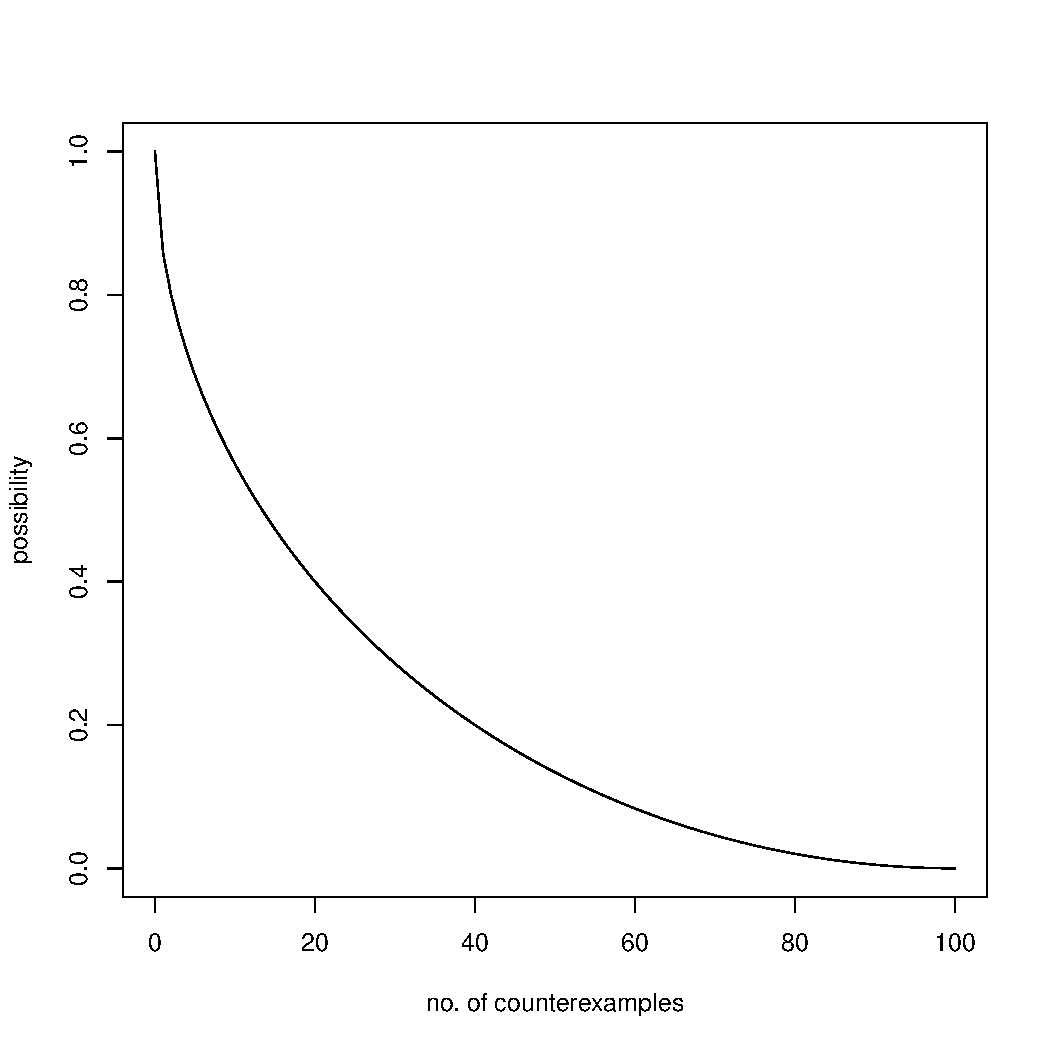
\includegraphics[width=2.25in]{../possibility} &
%      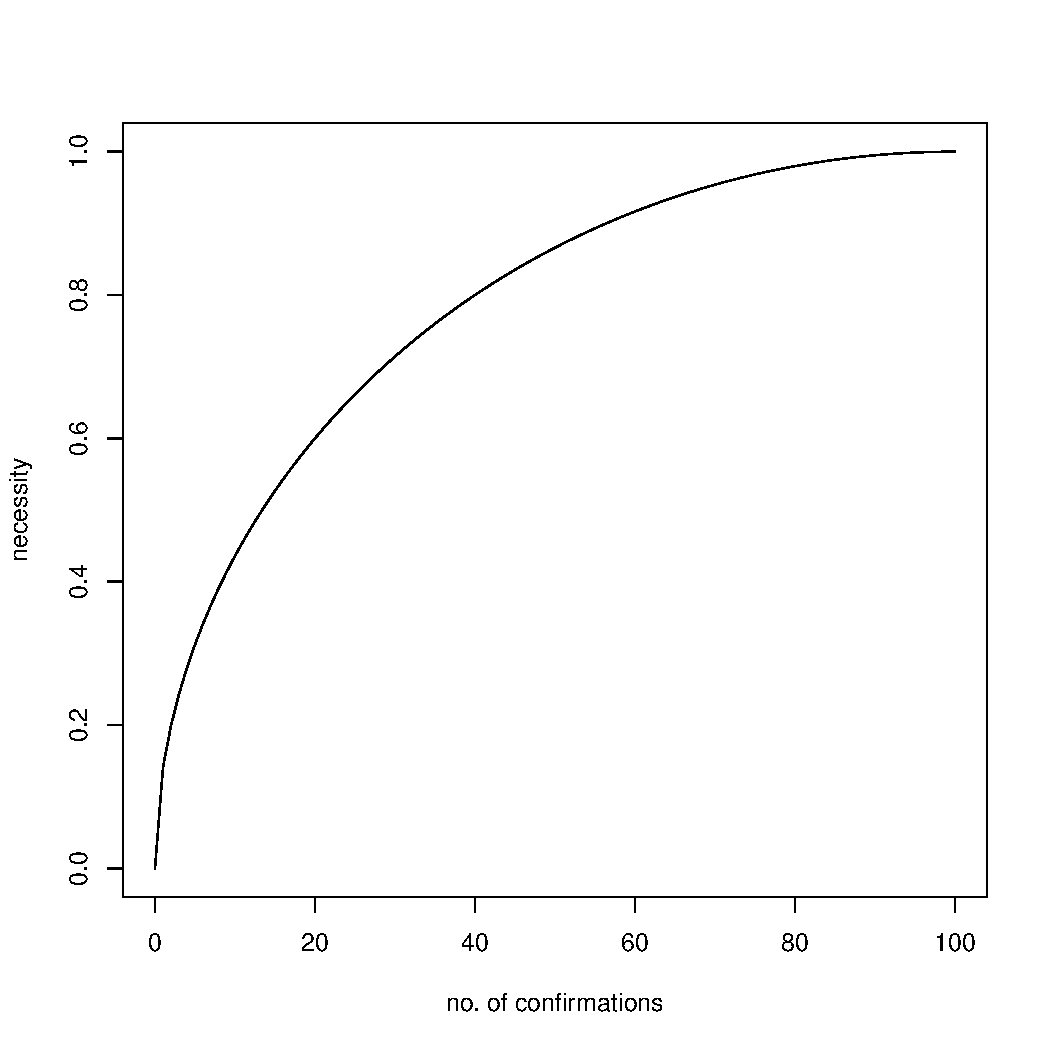
\includegraphics[width=2.25in]{../necessity} \\
%      (a) & (b)
%    \end{tabular}
%  \end{center}
%  \caption{A plot of $\Pi(\phi)$  as a function of
%    $u_\phi^-$ (a) and of $N(\phi)$ as a function of
%    $u_\phi^+$ (b) when $u_\phi = 100$.\label{fig:poss-nec-plots}}
%\end{figure}

\subsection{Axiom Scoring}
We combine the possibility and necessity of an axiom to define
a single handy acceptance/rejection index (ARI) as follows:
\begin{equation}\label{eq:ARI}
  \mathrm{ARI}(\phi) = N(\phi) - N(\neg\phi) = N(\phi) + \Pi(\phi) - 1 \in [-1, 1].
\end{equation}
A negative $\mathrm{ARI}(\phi)$ suggests rejection of $\phi$ ($\Pi(\phi)<1$),
whilst a positive $\mathrm{ARI}(\phi)$ suggests its acceptance ($N(\phi)>0$),
with a strength proportional to its absolute value. A value close to zero
reflects ignorance about the status of $\phi$.

Although this ARI is useful for the purpose of analyzing the results of our
experiments and to visualize the distribution of the tested axiom with respect
to a single axis, one should always bear in mind that an axiom is scored by
the proposed heuristics in terms of two bipolar figures of merit,
whose meanings, though related, are very different:
\begin{itemize}
\item $\Pi(\phi)$ expresses the degree to which $\phi$ may be considered ``normal'',
  in the sense of ``not exceptional, not surprising'', or not contradicted by
  actual observations;
\item $N(\phi)$, on the other hand, expresses the degree to which $\phi$ is
  certain, granted by positive evidence and corroborated by actual observations.
\end{itemize}


\section{A Framework for Candidate Axiom Testing}
\label{OWL2SPARQL} 



%The semantics of the 32 axiom types of OWL~2 may be taken as a starting point to define,
%for each axiom type, which facts recorded in a given RDF triple store are to be taken as
%supporting evidence, or \emph{confirmations} of the axiom and which facts are to be
%construed as refuting evidence, or \emph{counterexamples}, based on the principles
%laid out in Section~\ref{epistemology}.

A general algorithm for testing all the possible OWL~2 axioms in a given RDF store is beyond the scope of this paper. 
Here, we will restrict our attention to \texttt{Class} and \texttt{ObjectComplementOf} class expressions and to \texttt{SubClassOf} axioms. 
Scoring these axioms with their ARI requires to compute the interpretation of \texttt{Class} and \texttt{ObjectComplementOf} class expressions. 
 
\subsection{Computational Definition of \texttt{Class} and \texttt{ObjectComplementOf} Class Expressions}
We define a mapping $Q(E, \mbox{\tt ?x})$ from OWL~2 class expressions to SPARQL graph patterns,
where $E$ is an OWL~2 class expression, and $\mbox{\tt ?x}$ is a variable,
such that the query
\texttt{SELECT DISTINCT ?x WHERE \{} $Q(E, \mbox{\tt ?x})$ \texttt{\}}
returns all the individuals which are instances of $E$. We denote this set by
$[Q(E, \mbox{\tt ?x})]$:
\begin{equation}
[Q(E, \mbox{\tt ?x})] = \{ v : (?x, v) \in ResultSet(\mbox{\tt SELECT DISTINCT ?x WHERE} \{ Q(E, \mbox{\tt ?x}) \} \}.
\end{equation} 

For a \texttt{Class} class expression $A$ (i.e., an atomic concept in DL), 
\begin{equation}
Q(A, \mbox{\tt ?x}) = \{\mbox{\tt ?x a }A \},
\end{equation}
where $A$ is a valid IRI.

For an \texttt{ObjectComplementOf} class expression, things are slightly more complicated, since RDF does not support
negation. The model-theoretic semantics of OWL class expressions of the form \texttt{ObjectComplementOf(}$C$\texttt{)}
($\neg C$ in DL syntax), where $C$ denotes a class, is $\Delta^\mathcal{I} \setminus C^\mathcal{I}$.
However, to learn axioms from an RDF dataset, the open-world hypothesis must be made: the absence of
supporting evidence does not necessarily contradict an axiom, moreover an axiom might
hold even in the face of a few counterexamples.
%For example, for 143 out of 541 \texttt{SubClassOf} axioms in the DBpedia
%ontology, no resource in the DBpedia dataset provides any evidence;
%for 28, at least one counterexample is found in DBpedia 3.9.
%Axiom \texttt{SubClassOf(dbo:Person dbo:Agent)} even has 76 counterexamples!
%\todo{voir si on veut virer le paragraphe ci-dessus}
Therefore, as proposed in~\cite{TettamanziFaronZuckerGandon2014ekaw}, we define
$Q(\neg C, \mbox{\tt ?x})$ as follows, to approximate an open-world semantics:
\begin{equation}\label{eq:approx-open-world-negation}
  Q(\neg C, \mbox{\tt ?x}) =
  \begin{minipage}[t]{2in}
    \begin{tabbing}
      \quad\=\quad\=\quad\=\kill
      \{\>\texttt{?x a ?dc .}\\
        \>\texttt{FILTER NOT EXISTS} \{ \texttt{?z a ?dc . } $Q(C, \mbox{\tt ?z})$ \texttt{\} \}},
    \end{tabbing}
  \end{minipage}
\end{equation}
where \texttt{?z} is a variable that does not occur anywhere else in the query.

For an atomic class expression $A$, this becomes
%\begin{equation}
%Q(\neg A, \mbox{\tt ?x}) =
%  \begin{minipage}[t]{3in}
%    \begin{tabbing}
%      \quad\=\quad\=\quad\=\kill
%      \{\>\texttt{?x a ?dc .}\\
%        \>\texttt{FILTER NOT EXISTS} \{\\
%        \>\>\texttt{?z a ?dc . ?z a} $A$ \texttt{\} \}},
%    \end{tabbing}
%  \end{minipage}
%\end{equation}
\begin{equation}
Q(\neg A, \mbox{\tt ?x}) = \{\>\texttt{?x a ?dc . } \mbox{\tt FILTER NOT EXISTS } \{ \mbox{\tt ?z a ?dc . ?z a }A \} \}.
\end{equation}


\subsection{Computational Definitions of the Support and the ARI of \texttt{SubClassOf} Axioms}
\label{comp-def-content}

The semantics of \texttt{SubClassOf} axioms of the form $C~\sqsubseteq~D$ is $C^\mathcal{I} \subseteq D^\mathcal{I}$,
which may also be written $x \in C^\mathcal{I} \Rightarrow x \in D^\mathcal{I}$.
Therefore, according to Equation~\ref{eq:support} and
%\begin{equation}
%u_{C \sqsubseteq D} = \| \{ r \in [ \mbox{ ?x a C } ] \Rightarrow r \in [ \mbox{ ?x a D } ] : r \mbox{  occuring in the RDF dataset } \} \|.
%\end{equation}
following the principle of selective confirmation,
\begin{equation}
%  u_{C \sqsubseteq D} = \| \{D(a) : \mbox{$C(a)$ in the RDF dataset} \} \|,
  u_{C \sqsubseteq D} = \| \{D(a) : \mathcal{K} \models C(a) \} \|,
\end{equation}
because, if $C(a)$ holds, then $C(a) \Rightarrow D(a) \equiv \neg C(a) \lor D(a) \equiv \bot \lor D(a) \equiv D(a)$.

\noindent
As a result, a computational definition of $u_{C \sqsubseteq D}$ is the following SPARQL query:
\begin{equation}
  \begin{minipage}[c]{5in}
    \begin{tabbing}
      \quad\=\quad\=\quad\=\kill
      \texttt{SELECT (count(DISTINCT ?x) AS ?u)}\\
      \texttt{WHERE} \{$Q(C, \mbox{\tt ?x})$\}.
    \end{tabbing}
  \end{minipage}
\end{equation}


In order to compute the score of \texttt{SubClassOf} axioms, $ARI(C \sqsubseteq D)$, we must provide a computational definition of $u^+_{C \sqsubseteq D}$ and $u^-_{C \sqsubseteq D}$. We start with the following statements:
\begin{itemize}
\item confirmations are individuals $i$ such that
  $i \in [Q(C, \mbox{\tt ?x})]$ and $i \in [Q(D, \mbox{\tt ?x})]$;
\item counterexamples are individuals $i$ such that
  $i \in [Q(C, \mbox{\tt ?x})]$ and $i \in [Q(\neg D, \mbox{\tt ?x})]$.
\end{itemize}
This may be translated into the following two SPARQL queries to compute $u^+_{C \sqsubseteq D}$ and $u^-_{C \sqsubseteq D}$ respectively:
\begin{equation}
  \begin{minipage}[c]{5in}
    \begin{tabbing}
      \quad\=\quad\=\quad\=\kill
      \texttt{SELECT (count(DISTINCT ?x) AS ?nConfirm)}\\
      \texttt{WHERE} \{ $Q(C, \mbox{\tt ?x})$ $Q(D, \mbox{\tt ?x})$ \}
    \end{tabbing}
  \end{minipage}
\end{equation}
and
\begin{equation}
  \begin{minipage}[c]{5in}
    \begin{tabbing}
      \quad\=\quad\=\quad\=\kill
      \texttt{SELECT (count(DISTINCT ?x) AS ?nCounter)}\\
      \texttt{WHERE} \{ $Q(C, \mbox{\tt ?x})$ $Q(\neg D, \mbox{\tt ?x})$ \}.
    \end{tabbing}
  \end{minipage}
\end{equation}
Notice that an $i$ such that $i \in [Q(C, \mbox{\tt ?x})]$ and $i \notin [Q(D, \mbox{\tt ?x})]$
does not contradict $C \sqsubseteq D$, because it might well be the case
that the assertion $D(i)$ is just missing.
Likewise, an $i \in [Q(\neg D, \mbox{\tt ?x})]$ such that $i \in [Q(\neg C, \mbox{\tt ?x})]$
will not be treated as a confirmation, based on our choice to regard as
evidence in favor of a hypothesis only selective confirmations.



\subsection{Heuristics based on Time Capping}

The results of our first experimentation described in the following Section~\ref{evaluation}
show that the time it takes to test an axiom tends to be upper bounded 
%Fabien: without any factor? the formulation sounds strange as if the two quantities were directly comparable.
%cath: cela fait 2 fois qu'un relecteur est gêné par ce upper bounded (un reviewer déjà)... mais je ne sais pas quoi changer
by the inverse
of $1 + \mathrm{ARI}(\phi)$: an axiom which takes too long to test will likely end up having a very negative score.
We defined two heuristics based on this idea.
\begin{itemize}
%Fabien: intéressante subtilité:
%le graphique colorié (l'analyse comparative avec possibility) montre bien le premier point mais pas le deuxième.
%cath: on l'a viré ce graphique, il faut qu'on le montre autrement
%pour cela il faudrait associer une couleur allant de vert à jaune mais cette fois avec vert pour les axiomes ont été trouvé au début de la session de calcul et jaune pour celles qui ont été trouvées à la fin afin de voir la progression dans l'espace de recherche.
%cath: en fait il semble que ce ne sois pas très pertinent comme heuristique au vu du dernier graphique produit alors qu'on avait vu que si il y a un certain temps... je ne comprends plus rien mais il est tard.
\item We time-cap the SPARQL queries to compute the ARI of a candidate axiom and decide whether to accept or reject it, since above a computation time threshold, the axiom being tested is likely to get a negative ARI and be rejected.
\item We construct candidate axioms of the form $C \sqsubseteq D$, by considering
the subclasses $C$ in increasing order of the number of classes $D$ sharing at least
one instance with $C$.
This enables us to maximize the number of tested and accepted axioms in a given time period,
since it appears that the time it takes to test $C \sqsubseteq D$ increases with that number
and the lower the time, the higher the ARI.
\end{itemize}

%In statistics, \emph{censoring} is when the value of a measurement or observation
%is not known for some sample points. A sample contains censored observations
%if the only information about some of the observations is that they are below
%or above a specified value.
%
% NIST/SEMATECH e-Handbook of Statistical Methods, http://www.itl.nist.gov/div898/handbook/, Jan 11, 2015
% http://www.itl.nist.gov/div898/handbook/apr/section1/apr131.htm
%
% Chapter 11, Analyzing Below Detection-limit data, from Millard, Dixon, and Neerchal, Environmental Statistics with R
% http://www.public.iastate.edu/~pdixon/stat505/Chapter%2011.pdf

%Here, we use this concept to refer to the fact that, when testing an OWL axiom,
%if one caps the time the test should take, the exact value of the score
%for the axiom whose test times out will not be known.
%From a statistical point of view, this produces a random censoring,
%because both the number of censored observations and the censoring levels
%are random outcome.

\section{Evaluation on \texttt{SubClassOf} Axiom Testing}
\label{evaluation}


\subsection{Experimental Protocol}

We evaluated the proposed scoring heuristics by performing tests of subsumption
axioms using DBpedia 3.9 in English as the reference RDF fact repository.
In particular, on April 27, 2014, we downloaded the DBpedia dumps of English version 3.9,
generated in late March/early April 2013, along with the DBpedia ontology, version 3.9.
This local dump of DBpedia, consisting of 812,546,748 RDF triples,
has been bulk-loaded into Jena TDB and a prototype
for performing axiom tests using the proposed method has been coded in Java,
using Jena ARQ and TDB to access the RDF repository.

We systematically generated and tested subsumption axioms
involving atomic classes only according to the following protocol:
for each of the 442 classes $C$ referred to in the RDF repository,
we construct all axioms of the form $C \sqsubseteq D$ such that $C$ and $D$
share at least one instance. Classes $D$ are obtained with the following query: 

\[
  \mbox{\tt SELECT DISTINCT ?D WHERE} \{ Q(C, \mbox{\tt ?x}) \mbox{\tt\ . ?x a ?D} \}.
\]

Experiments have been performed on two machines:
\begin{itemize}
\item a Fujitsu CELSIUS workstation equipped
with twelve six-core Intel Xeon CPU E5-2630 v2 processors at 2.60GHz clock speed,
with 15,360 KB cache each, 128 GB RAM,
4 TB of disk space with a 128 GB SSD cache,
under the Ubuntu  12.04.4 LTS 64-bit operating system;
\item a HP  portable PC equipped
% according to the /proc/cpuinfo file on TOMTY
with four two-cores Intel\textregistered\ Core\texttrademark\ i7-4600U CPUs at 2.10GHz clock speed,
with a 4,096 KB cache, 16 GB RAM,
128 GB of disk space,
under the Fedora 64-bit Linux operating system.
\end{itemize}
The former was used to test 644 axioms without time capping.
The latter, much less powerful but representative of a common high-end laptop computer,
was then used to obtain the results with time capping.




\subsection{Results without Time Capping}
\label{results-no-timeout}




%cath si on veut garder l'analyse comparative dans un futur article cela sera un paragraphe à part
%cath et il faudra prendre en compte la remarque du reviewer 1 d'eswc2015:
%reviewer 1: it is not really clear how the accuracy was measured (i.e., why the proposed ARI index is more accurate than the probabilistic score) 

%Figure~\ref{fig:ARI-BLS} compares the results obtained in this preliminary experiment
%to the probabilistic score proposed in~\cite{BuehmannLehmann2012}.
%As already discussed in~\cite{TettamanziFaronZuckerGandon2014ekaw}, the proposed
%acceptance-rejection index is more accurate than the probabilistic score.
%However, its increased accuracy comes at a higher computational cost.
%The two heuristics, time capping and candidate axioms ordering, make up for it (see Section \ref{results-timeout}).

%Cath ne pas faire référence aux couleurs dans les explications de graphiques car impressions noir et blanc

%\begin{figure}[t]
%\begin{center}
%    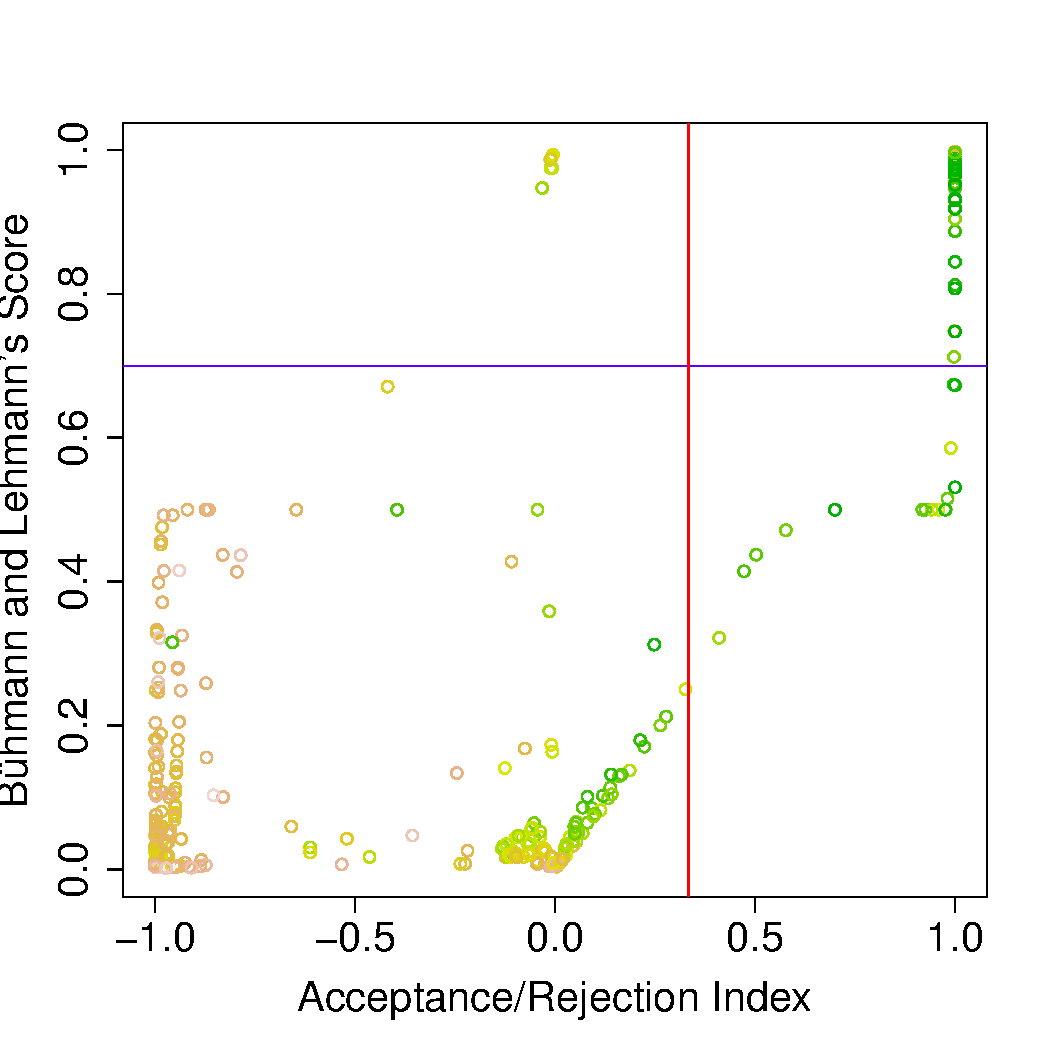
\includegraphics[height=2.5in]{ARI-BLS}
%\end{center}
%\caption{A comparison of the acceptance/rejection index and the probability-based
%  score used in~\cite{BuehmannLehmann2012} on axioms tested without time capping.
%  The vertical line shows the acceptance threshold $\mathrm{ARI}(\phi)>1/3$;
%  the horizontal line the acceptance threshold of 0.7 for the probabilistic score.}
%\label{fig:ARI-BLS}
%\end{figure}
%
%\begin{figure}[t]
%\begin{center}
%    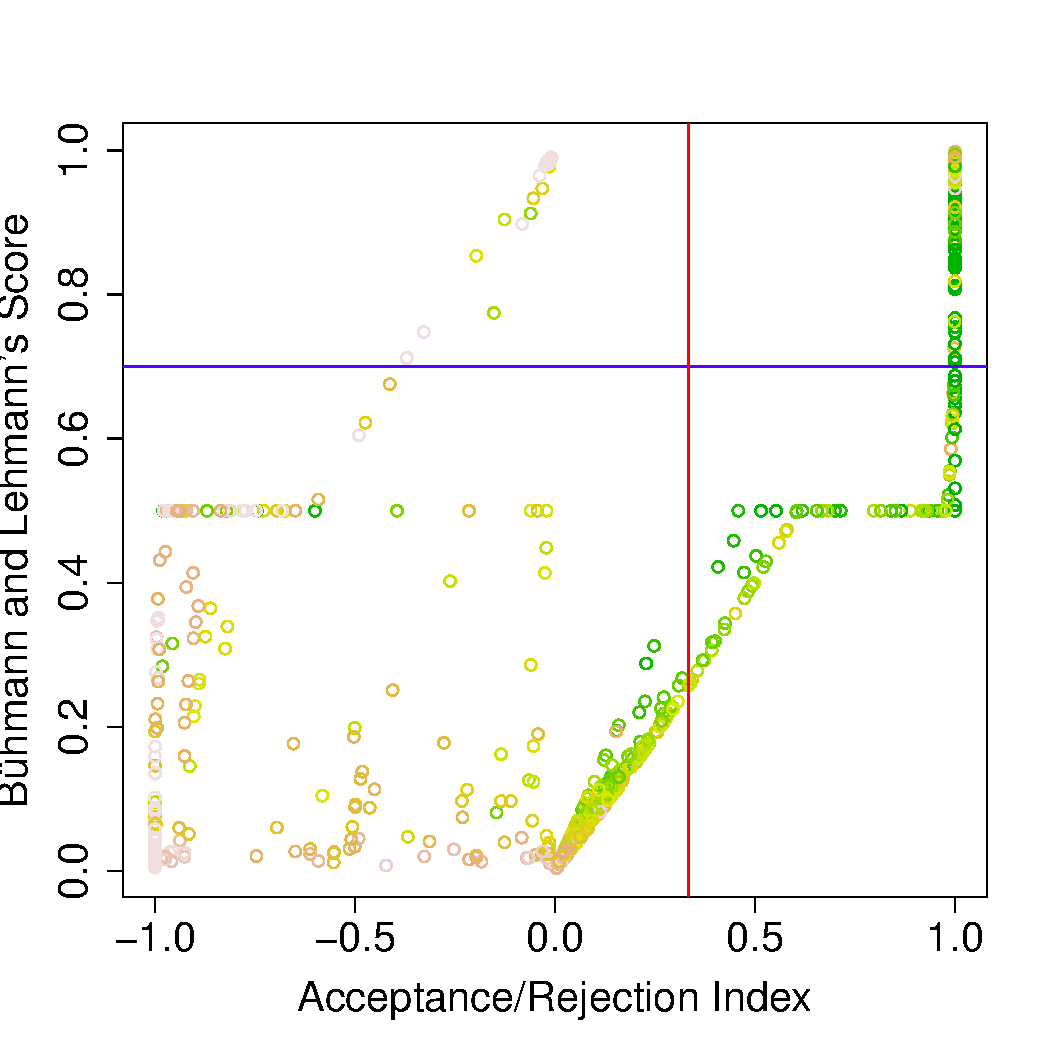
\includegraphics[height=2.5in]{ARI-BLS-20}
%\end{center}
%\caption{A comparison of the acceptance/rejection index and the probability-based
%  score used in~\cite{BuehmannLehmann2012} on axioms tested with a 20-minute time cap.
%  The vertical line shows the acceptance threshold $\mathrm{ARI}(\phi)>1/3$;
%  the horizontal line the acceptance threshold of 0.7 for the probabilistic score.}
%\label{fig:ARI-BLS-20}
%\end{figure}


\begin{figure}[t]
\begin{center}
  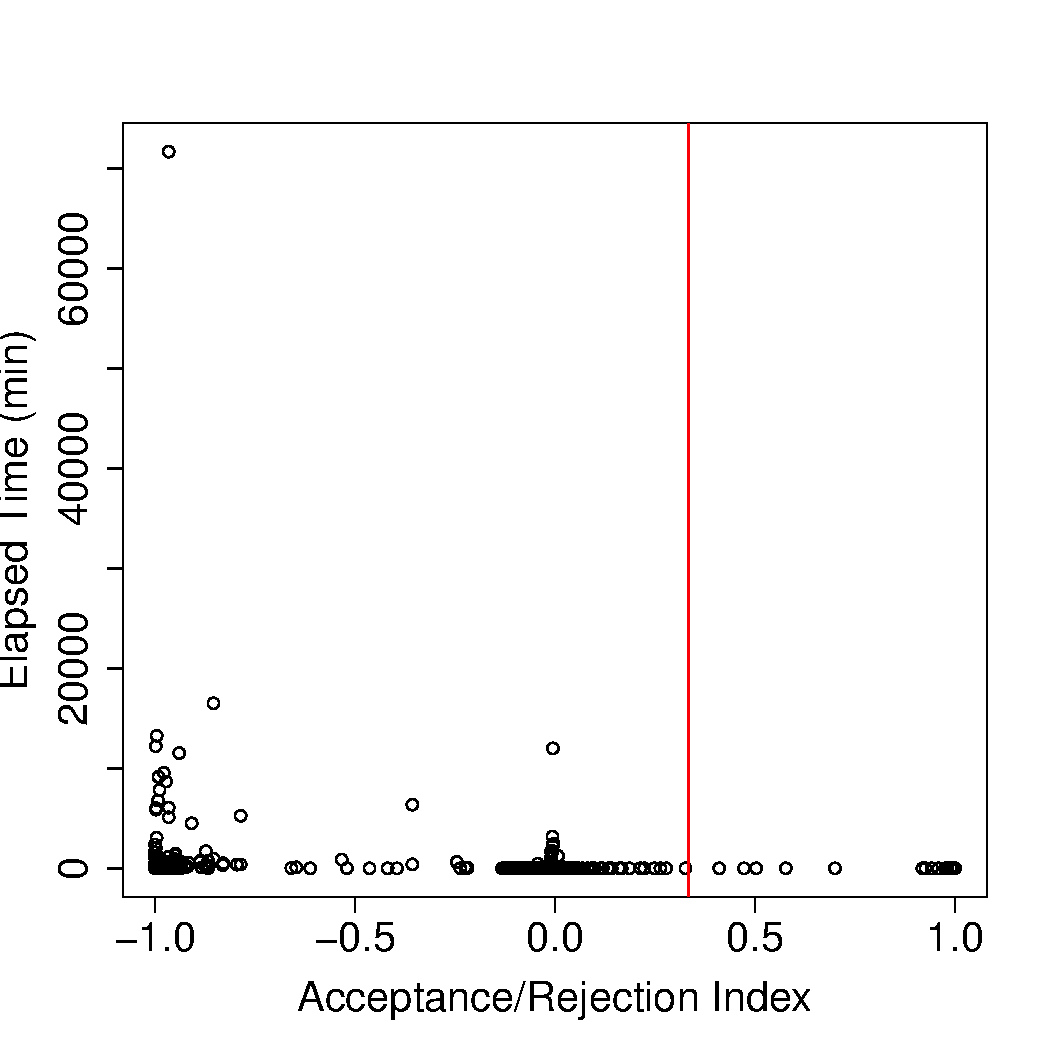
\includegraphics[height=2.5in]{time-ARI}
\end{center}
\caption{Plot of the time taken for testing the systematically generated
 \texttt{SubClassOf} axioms without time capping as a function of ARI.
  The vertical line shows the acceptance threshold $\mathrm{ARI}(\phi)>1/3$.}
\label{fig:time-ARI}
\end{figure}

We managed to test 644 axioms without time capping.
The results of this first experiment
show that the time it takes to test an axiom tends to be inversely proportional
to its score (see Figure~\ref{fig:time-ARI}): an axiom which takes
too long to test will likely end up having a very negative score.
If we restrict our attention to the 197 axioms with an ARI above the
acceptance threshold empirically set at $1/3$ in~\cite{TettamanziFaronZuckerGandon2014ekaw},
we discover that the average elapsed time for testing them is 20.5~s,
the median time is 156~ms, and the longest elapsed time is 1584.3~s, or 26~min 24~s.
Out of the 197 accepted axioms,
135 (68.5\%) were tested in less than 1~s,
165 (83.75\%) in less than 10~s,
187 (95\%) in less than 1~minute,
and 195 (99\%) in less than 10~minutes.

Altogether, testing those 644 axioms took a staggering 20,328,791,473~ms (= 235~days 6~h 53~min 11.473~s).
If all tests had been time-capped to exactly 10 minutes, the total elapsed time
would have been ``just'' 182,481,760~ms (= 2 days 2~h 41~m 21.76~s),
i.e., less than 0.9\% of the actual time, with a two orders of magnitude speedup!


\subsection{Results with Time Capping}
\label{results-timeout}


\begin{figure}[t]
\begin{center}
  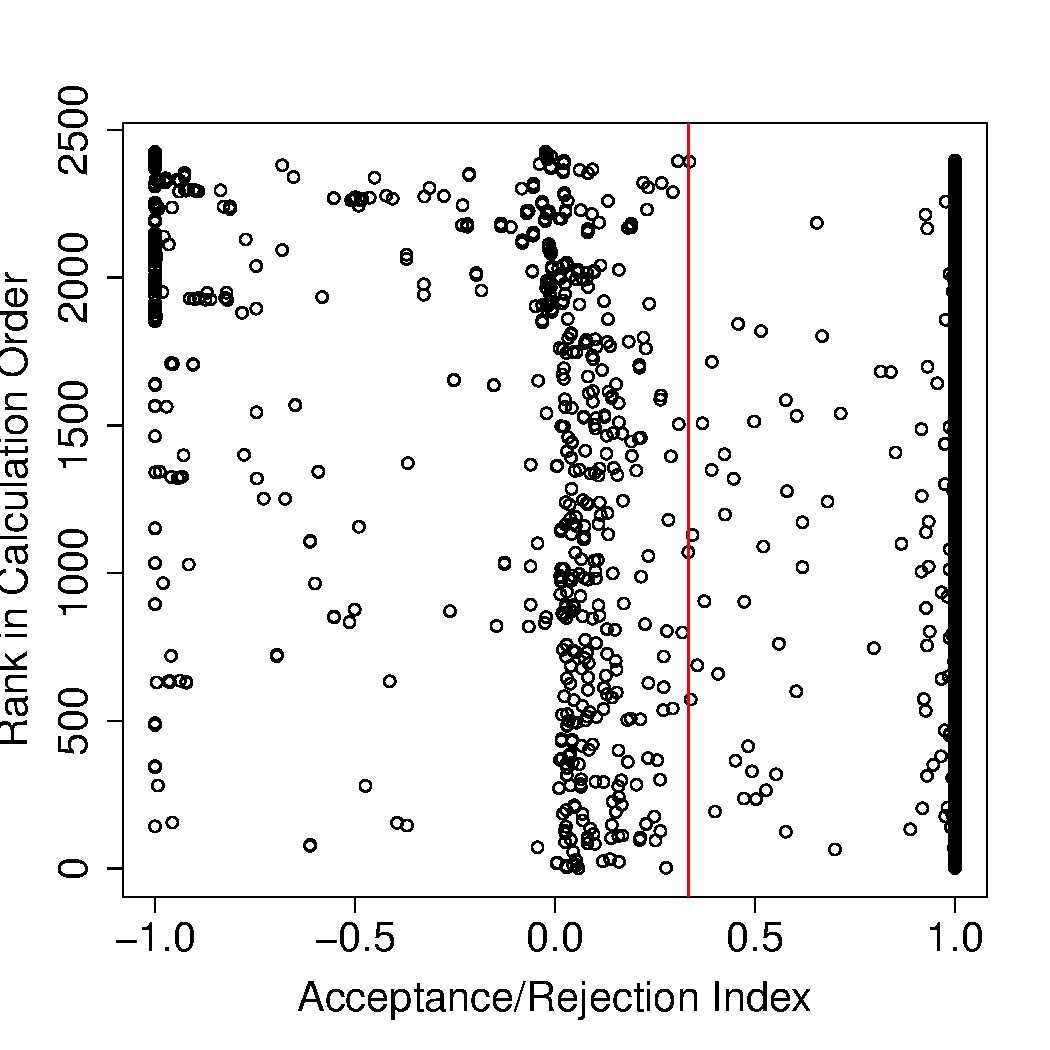
\includegraphics[height=2.5in]{rank-ARI-20}
\end{center}
\caption{Plot of the rank in the testing order for the systematically generated
 \texttt{SubClassOf} axioms with time capping as a function of ARI.
  The vertical line shows the acceptance threshold $\mathrm{ARI}(\phi)>1/3$.}
\label{fig:rank-ARI}
\end{figure}

Based on these observations, we decided to fix to 20 min
(i.e., twice the time it took to test 99\% of the accepted axioms on the more powerful machine)
the threshold to time-cap the SPARQL queries to compute $u^+_{C \sqsubseteq D}$ and $u^-_{C \sqsubseteq D}$
in order to decide whether to accept or reject a candidate axiom $C \sqsubseteq D$.

For this new round of experiments, we used the candidate axiom ordering heuristics
in order to get as much tested axioms as possible.
Figure \ref{fig:rank-ARI} shows the distribution of axioms depending on their ARI
and their rank in the calculation ordering. The concentration of axioms with both a high rank and an ARI equal to $-1$ confirms the interest of our heuristics of candidate axiom ordering.


Thanks to the greatly reduced overhead,
%(cf.\ Figure~\ref{fig:time-ARI-20}),
we were able to test 2,426 axioms at the time of writing. 
%The results are shown in Figure~\ref{fig:ARI-BLS-20}.
% Number of time-capped axioms:
% dim(d20[d20$time > 1200000 & d20$refc==(d20$conf + d20$expt) & d20$ari<1/3,])[1]
Among them, 197 axioms have been time-capped (and therefore rejected).
A qualitative analysis of the results (see Section~\ref{qualitative}) shows that
43 out of them should have been accepted.
%\todo{update the above sentence with the exact error rate. In fact it would have been better to test the 197 axioms to evaluate the difference between both algos, independently of the qualitative analysis}
This represents an error rate of less than 1.8\%. If we take into account the dramatic
improvement in terms of speed, this looks like a very reasonable price to pay
in terms of accuracy degradation. In addition, it should be observed that,
by construction, the errors are all in the same direction, i.e., some axioms
which should be accepted are in fact rejected: at least, this is a conservative
heuristics, since it does not generate false positives.

\subsection{Qualitative Analysis of the Results}
\label{qualitative}

Among the 2,426 candidate axioms automatically tested, 1,650 axioms are accepted (and 776 are rejected).
Among them, 331 are already in the DBpedia ontology, 344 are trivial
(i.e., tautologies of the form \texttt{SubClassOf(\dots\ owl:Thing)}), then 975 are novels axioms.
This means that our method has the potential to discover large numbers of novel axioms.

A human analysis of the results of the automatic process shows that out of the 2,426 candidate axioms which were tested, 204 are questionnable, i.e. $8.3\%$ of the results. 55 rejected axioms (scored by the system with an ARI value under the acceptance threshold) may be false negative and 149 accepted axioms (scored by the system with an ARI value above the acceptance threshold) may be false positives. 

The close analysis of the possibly 55 false negative led to the following conclusions. 
\begin{itemize}

\item 43 of them are time-capped axioms.
We tested these 43 time-capped false negatives without time capping, for comparison,
and we found that 13 of them (of which 5 tautologies) would have been accepted
if the test had not been interrupted; the remaining 30, however, would have been rejected anyway,
albeit with an ARI around zero, thus not strongly.
Whith respect to the total number of time-capped axioms (197), this represents an error rate of 6.6\%,
which is not bad, given the blunt character of the heuristics.
\item Among the 12 remaining false positives, 4 of them have a positive ARI (under the acceptance threshold). This may lead to the reasonable conclusion that the candidate axioms rejected with an ARI close to the acceptance threshold should always be examined by an ontologist. The 7 remaining axioms involve very general classes as superclass, e.g., \texttt{dbo:Person}, \texttt{dbo:Product}. Their low scoring may be the result of incomplete knowledge due to the fact that people populating the DBpedia ontology will focus on more specific classes.
These conclusions are in line with the results of the analysis of the negative scoring of 28 out of the 541 \texttt{SubClassOf} axioms in the DBpedia Ontology reported in \cite{TettamanziFaronZuckerGandon2014ekaw}. These negative scores are due to the presence of erroneous facts in the DBpedia dataset: instances of the subclass that also belong to a class disjoint with the superclass, e.g., \texttt{:USA} is both an instance of \texttt{dbo:LaunchPad} and \texttt{dbo:Country} which has no instance in common with \texttt{dbo:Infrastructure}; it thus contradicts axiom \texttt{dbo:LaunchPad} $\sqsubseteq$ \texttt{dbo:Infrastructure}. 
\end{itemize}


Conversely, the analysis of the 148 possibly false positives led to the following conclusions:
\begin{itemize}
\item Most of these axioms which should be rejected are inverted \texttt{subClassOf} relations
(e.g., \texttt{dbo:Case} $\sqsubseteq$ \texttt{dbo:LegalCase} instead of \texttt{dbo:LegalCase} $\sqsubseteq$ \texttt{dbo:Case}).
This occurs when counterexamples are missing (all instances of a class are instances of the other class too and the two axioms are positively scored).
%other inverted subClassOf relations: between dbo:SportManager and SoccerManager, dbo:ClericalAdministrativeRegion and dbo:Diocese, dbo:Region and dbo:AdministrativeRegion

\item The acceptance of some axioms involving vague concepts is questionable.
For instance, it seems that anything that can appear on a map could be typed with
\texttt{gml:\_Feature} and, therefore, many classes should be subclasses of it,
but it is not clear whether this is correct or not.
The same remark applies to \texttt{SubclassOf} axioms with class \texttt{dbo:Place} as superclass.

\item Some axioms involve concepts used in a more general sense than it could be expected.
Their acceptance is therefore dubious. It is for instance the case of \texttt{dbo:PokerPlayer}~$\sqsubseteq$~\texttt{dbo:Athlete}. Accepting it is not really a mistake in the sense that there are several other such concepts involving \texttt{dbo:Athlete}, e.g., \texttt{dbo:FigureSkater}~$\sqsubseteq$~\texttt{dbo:Athlete}. These axioms are acceptable when considering \texttt{dbo:Athlete} in its general sense.

\item Other questionable axioms are those involving a concept having at least two senses, e.g., \texttt{dbo:Library}, designating both a building and an institution. The joint acceptance of axioms \texttt{schema:Library}~$\sqsubseteq$~\texttt{dbo:Organisation} and \texttt{schema:Library}~$\sqsubseteq$~\texttt{dbo:Place} is not satisfactory.

\item Other questionable axioms are those involving a concept used both as a zoological class name, a taxon, and therefore marked as subclass of \texttt{dbp:Species}, and as a set of animals and, therefore, subclass of \texttt{dbo:Animal} and\break\texttt{dbo:Eukaryote}.
This is for instance the case of \texttt{dbo:Insect}.

\item The same confusion between the instance level and the ontological level
explains why most of the axioms involving \texttt{skos:Concept} should be rejected,
e.g., \texttt{dbo:Activity}~$\sqsubseteq$~\texttt{skos:Concept} or
\texttt{dbo:Train}~$\sqsubseteq$~\texttt{skos:Concept}.

%pb de modélisation sur domaines de pointe: en biologie, en juridique (SupremeCourtOfTheUnitedStatesCase)

\end{itemize}

If we define \emph{precision} as the fraction of the accepted axioms that is confirmed by the ontologist
and \emph{recall} as the fraction of the true axioms that is discovered by our axiom-scoring heuristics,
then one might argue that the recall of our heuristics is very promising,
while its precision needs to be improved.
However, as our previous discussion suggests, any improvement would depend more on the quality
of the RDF dataset than on the heuristics \emph{per se}.


To sum up, 
the high scoring of most of the candidate axioms which should be rejected
is due to misconceptions in the DBpedia RDF base or misuses of the DBpedia ontology by people populating it.
%\todo{contrairement \`a ce qu'on pensait, ceux qui sont discutables ne sont pas forc\'ement ceux avec peu de confirmations}




\section{Conclusion}\label{conclusion}

We have presented a possibilistic axiom scoring heuristics which is a viable
alternative to statistics-based heuristics. We have tested it by applying it to the
problem of testing \texttt{SubClassOf} axioms against the DBpedia database.
We have also proposed additional heuristics to greatly reduce its computational
overhead, consisting of setting a time-out on the test of each axiom and ordering the candidate axioms according to their score in order to optimize the number of axioms tested in a given time period.

Our results strongly support the validity of our hypothesis
that it is possible to alleviate the computation of the ARI without loosing too much
in terms of accuracy.

In addition, the qualitative analysis of the results confirm the interest of using axiom scoring heuristics like ours
not only to learn axioms from the LOD, but also to drive the validation and debugging of ontologies and RDF datasets.

Future work includes continuing our experiments by testing our algorithm on domain specific datasets
and extending it to learn other types of OWL axioms, beginning with \texttt{SubObjectPropertyOf} and \texttt{SubDataPropertyOf} axioms and \texttt{SubClassOf} axioms involving \texttt{ObjectSomeValuesFrom} class expressions.
%\section*{Acknowledgment}




\bibliographystyle{tetta-lncs}
\bibliography{../RDFMining}

\end{document}


